% \documentclass{article}
% \usepackage{NeededPackages}


% \title{ATmega328P - ADC}
% \author{Narendiran S}
% \date{\today}

% \begin{document}
% \maketitle

\section{Features}
\begin{itemize}
    \item 10-bit successive approximation ADC
    \item 65 to 260 $\mu$s conversion time
    \item 15 kilo samples per second
    \item 6 Multiplexed single ended input channels
    \item 2 Additional multiplexed single ended input channels depending on the package
    \item Temperature Sensor input Channel
    \item Selectable 1.1V ADC reference voltage
    \item Free running or singe conversion mode
    \item Interrupt on ADC conversion complete
\end{itemize}
\section{Overview}
\begin{itemize}
    \item Minimum value = 0V and Maximum value = $V_{REF}$ – 1 LSB
    \item $AV_{CC}$ can should be $V_{CC} \pm$ 0.3V.
    \item The \bitFormat{MUX} bits in \regFormat{ADMUX} register is used to select either ADC input pins or GND or Temperature Sensor or fixed band gap voltage reference(1.1V) for single ended input of ADC.
    \item The input clock frequency of ADC must be between 50kHz and 200kHz for max. resolution.
    \item Normal conversion takes 13 ADC clock cycles.
    \item The adc output are stored in \regFormat{ADCH} and \regFormat{ADCL} register.
    \item Can choose output between left or right adjusted by \bitFormat{ADLAR} bit in ADMUX.
\end{itemize}

\textbf{Notes :} First read \regFormat{ADCH} and then read \regFormat{ADCL}.

\newpage
\section{Block Diagram}
\begin{figure}[H]
    \centering
    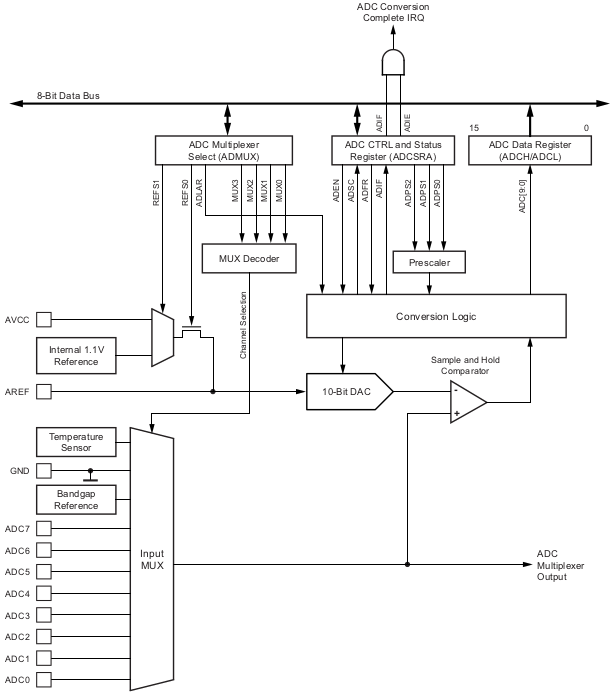
\includegraphics[height=0.75\textheight]{ADCBlock.png}
\end{figure}

\section{Starting Conversion}
\subsection{Single Conversion}
\begin{itemize}
    \item Disabling the power reduction ADC bit (\bitFormat{PRADC}).
    \item Writing logical one to ADC start conversion bit (\bitFormat{ADSC}).
    \item This Start conversion bit is cleared by hardware when ADC completes conversion.
\end{itemize}

\subsection{Triggered Conversion}
\begin{itemize}
    \item Many sources can be used to trigger.
    \item Auto trigger is enabled by setting ADC auto trigger enable bit(\bitFormat{ADATE}) in \regFormat{ADCSRA} register.
    \item Trigger source is selected by ADC trigger select bits (\bitFormat{ADTS}) in \regFormat{ADCSRB} register.
    \item When positve edge occur on selected trigger signal, the ADC starts conversion.
    \item Until the ADC conversion ends and another positve edge occur on selected trigger source, the next conversion wont's tart.
\end{itemize}

\subsubsection{Free Running Mode}
\begin{itemize}
    \item Using ADC interrupt Flag as trigger source makes the ADC start new conversion as soon as ongoing conversion ends.
    \item This is the free running mode, when constant sampling and updating is done.
    \item The first conversion is started by setting the \bitFormat{ADSC} bit \regFormat{ADCSRA} register.
    \item No need to clear interupt flag.
\end{itemize}

\textbf{Note :} The \bitFormat{ADSC} bit can be used to check if the conversion is going on or not independent of the mode.

\section{Register Description}
\subsubsection*{ADMUX – ADC Multiplexer Selection Register}
\vspace*{0.5cm}
\begin{bytefield}[bitformatting={\large\bfseries},
    endianness=big,bitwidth=0.125\linewidth]{8}
    \bitheader[lsb=0]{0-7} \\
    \bitbox{1}{\small REFS1}
    \bitbox{1}{\small REFS0}
    \bitbox{1}{\small ADLAR}
    \bitbox{1}{\small -}
    \bitbox{1}{\small MUX3}
    \bitbox{1}{\small MUX2}
    \bitbox{1}{\small MUX1}
    \bitbox{1}{\small MUX0}\\
\end{bytefield}

\begin{itemize}
    \item \bitFormat{ADLAR} - ADC Left Adjust Result - presentation of ADC conversion results.[1 - Left adjusted; 0 - Right adjusted]
\end{itemize}

\begin{table}[H]
    \begin{minipage}{0.318\textwidth}
        \centering
        \begin{tabular}{c|p{3.2cm}}
            \bitFormat{REFS[1:0]} & \textbf{Voltage Reference}\\
            \hline
            00 & AREF - the actual reference voltage\\
            01 & $AV_{CC}$\\
            10 & Reserved\\
            11 & Internal 1.1V\\
        \end{tabular}
    \end{minipage}
    \begin{minipage}{0.672\textwidth}
        \centering
        \begin{tabular}{c|c}
            \bitFormat{MUX[3:0]} & \textbf{Single Ended Input}\\
            \hline
            0000 & ADC0\\
            0001 & ADC1\\
            0010 & ADC2\\
            0011 & ADC3\\
            0100 & ADC4\\
            0101 & ADC5\\
            0110 & ADC6\\
            0111 & ADC7\\
            1000 & Temperature Sensor\\
            1110 & 1.1V Internal Voltage Reference\\
            111 & 0V\\
        \end{tabular}
    \end{minipage}
\end{table}

\subsubsection*{ADCSRA – ADC Control and Status Register A}
\vspace*{0.5cm}
\begin{bytefield}[bitformatting={\large\bfseries},
    endianness=big,bitwidth=0.125\linewidth]{8}
    \bitheader[lsb=0]{0-7} \\
    \bitbox{1}{\small REFS1}
    \bitbox{1}{\small REFS0}
    \bitbox{1}{\small ADLAR}
    \bitbox{1}{\small -}
    \bitbox{1}{\small MUX3}
    \bitbox{1}{\small MUX2}
    \bitbox{1}{\small MUX1}
    \bitbox{1}{\small MUX0}\\
\end{bytefield}

\begin{itemize}
    \item \bitFormat{ADEN} - ADC Enable - enabled the ADC.
    \item \bitFormat{ADSC} - ADC Start Conversion - starts the conversion in singe conversion mode and start first conversion in free running mode.
    \item \bitFormat{ADATE} - ADC Auto Trigger Enable - auto triggering the ADC on positve edge of selected trigger signal.
    \item \bitFormat{ADIF} - ADC Interrupt Flag - indicates the End of conversion.
    \item \bitFormat{ADIE} - ADC Interrupt Enable- enables the ADC conversion complete interrupt. 
\end{itemize}

\begin{table}[H]
    \centering
    \begin{tabular}{c|c}
        \bitFormat{ADPS[2:0]} \textbf{- ADC Prescaler Select} & \textbf{Division Factor}\\
        \hline
        000 & 2\\
        001 & 2\\
        010 & 4\\
        011 & 8\\
        100 & 16\\
        101 & 32\\
        110 & 64\\
        111 & 128\\
    \end{tabular}
\end{table}

\subsubsection*{ADCSRB – ADC Control and Status Register B}
\vspace*{0.5cm}
\begin{bytefield}[bitformatting={\large\bfseries},
    endianness=big,bitwidth=0.125\linewidth]{8}
    \bitheader[lsb=0]{0-7} \\
    \bitbox{1}{\small –}
    \bitbox{1}{\small ACME}
    \bitbox{1}{\small -}
    \bitbox{1}{\small -}
    \bitbox{1}{\small -}
    \bitbox{1}{\small ADTS2}
    \bitbox{1}{\small ADTS1}
    \bitbox{1}{\small ADTS0}\\
\end{bytefield}

\begin{table}
    \centering
    \begin{tabular}{c|c}
        \bitFormat{ADTS[2:0]} \textbf{- ADC Auto Trigger Source Selections} & \textbf{Trigger Source}\\
        \hline
        000 & Free running mode\\
        001 & Analog comparator\\
        010 & External interrupt request 0\\
        011 & Timer/Counter0 compare match A\\
        100 & Timer/Counter0 overflow\\
        101 & Timer/Counter1 compare match B\\
        110 & Timer/Counter1 overflow\\
        111 & Timer/Counter1 capture event\\
    \end{tabular}
\end{table}

\subsubsection*{ADCL and ADCH – The ADC Data Register}
\subsubsection*{ADLAR=0}
\vspace*{0.5cm}
\begin{bytefield}[bitformatting={\large\bfseries},
    endianness=big,bitwidth=0.125\linewidth]{8}
    \bitheader[lsb=8]{8-15} \\
    \bitbox{1}{\small -}
    \bitbox{1}{\small -}
    \bitbox{1}{\small -}
    \bitbox{1}{\small -}
    \bitbox{1}{\small -}
    \bitbox{1}{\small -}
    \bitbox{2}{\small ADC[9:8]}\\
    \bitbox{8}{\small ADC[7:0]}\\
    \\ 
    \bitheader[lsb=0]{0-7}\\
\end{bytefield}
\subsubsection*{ADLAR=1}
\vspace*{0.5cm}
\begin{bytefield}[bitformatting={\large\bfseries},
    endianness=big,bitwidth=0.125\linewidth]{8}
    \bitheader[lsb=8]{8-15} \\
    \bitbox{8}{\small ADC[9:2]}\\
    \bitbox{2}{\small ADC[1:0]}
    \bitbox{1}{\small -}
    \bitbox{1}{\small -}
    \bitbox{1}{\small -}
    \bitbox{1}{\small -}
    \bitbox{1}{\small -}
    \bitbox{1}{\small -}
    \\
    \\ 
    \bitheader[lsb=0]{0-7}\\
\end{bytefield}

\section{Configuring the ADC}
\subsection{Single Conversion}
\begin{itemize}
    \item First, Voltage Reference is choosen by configuring the \bitFormat{REFS[1:0]} bits in \regFormat{ADMUX} register.
    \item Next, the ADC output presentation either left or right adjusting is choosen by configuring the \bitFormat{ADLAR} bit in \regFormat{ADMUX} register.
    \item Next, the channel is choosen by configuring the \bitFormat{MUX[3:0]} bits in \regFormat{ADMUX} register.
    \item Next, for single conversion, the \bitFormat{ADATE} - ADC auto trigger bit is cleared in \regFormat{ADCSRA} register.
    \item Interrupt is disbaled, as we use single conversion every time in program by clearing the \bitFormat{ADIE} bit in \regFormat{ADCSRA} register.
    \item The Prescaler for ADC clock is choosen so that the clock is  between 50kHz and 200kHz  by Configuring the \bitFormat{ADPS[2:0]} bits in \regFormat{ADCSRA} register.
    \item ADC is enabled by seting the \bitFormat{ADEN} bit in \regFormat{ADCSRA} register.
    \item Finally, the ADC conversion is started by setting the \bitFormat{ADSC} bit in  \regFormat{ADCSRA} register.
    \item Next, we check the \bitFormat{ADSC} flag for end of conversion.
    \item We can read the output from \bitFormat{ADC} register.
\end{itemize}
\begin{minted}[breaklines, bgcolor=lightgray]{c}
DDRC &= ~(1<<channel_no);

// Selecting Voltage Referece
// Lets use AREF pin
// REFS[1:0] -- 00
ADMUX &= ~(1<<REFS0);
ADMUX &= ~(1<<REFS1);

// Selecting the Presentation of ADC output
// Right adjust - ADLAR == 0
ADMUX &= ~(1<<ADLAR);

// SELECTINT the channel for ADC
// LET'S select channel_no
// MUX[3:0]&0xF0 | channel_no
ADMUX = (ADMUX & 0XF0) | channel_no;

// for single conversion - disabling ADC auto trigger
// ADATE == 0
ADCSRA &= ~(1<<ADATE);

// disable the interrrupt by disbaling ADIE bit
// ADIE == 0
ADCSRA &= ~(1<<ADIE);

//  Prescaler be 64 so that we get 8Mhz/64 = 125kHz
// ADPS[2:0] -- 110
ADCSRA |= (1<<ADPS2) | (1<<ADPS1);
ADCSRA &= ~(1<<ADPS0);

// ENABLING adc
ADCSRA |= (1<<ADEN);

// STARTING CONVERSIOn
ADCSRA |= (1<<ADSC);

    // since single conversion, we can check start conversion bit
while((ADCSRA & (1<<ADSC)))
{
    
}
// RESSETTING THE Flag
// ADCSRA |= (1<<ADIF);
return ADC;
\end{minted}



\subsection{Free Running Conversion}
\begin{itemize}
    \item First, Voltage Reference is choosen by configuring the \bitFormat{REFS[1:0]} bits in \regFormat{ADMUX} register.
    \item Next, the ADC output presentation either left or right adjusting is choosen by configuring the \bitFormat{ADLAR} bit in \regFormat{ADMUX} register.
    \item Next, the channel is choosen by configuring the \bitFormat{MUX[3:0]} bits in \regFormat{ADMUX} register.
    \item Next, the trigger source of auto trigger is choosen by selecting 000 (free running) in \bitFormat{ADTS[2:0]} bits in \regFormat{ADCSRA} register.
    \item Next, for Free Running conversion, the \bitFormat{ADATE} - ADC auto trigger bit is set in \regFormat{ADCSRA} register.
    \item Interrupt is enabled by setting the \bitFormat{ADIE} bit in \regFormat{ADCSRA} register.
    \item The Prescaler for ADC clock is choosen so that the clock is  between 50kHz and 200kHz  by Configuring the \bitFormat{ADPS[2:0]} bits in \regFormat{ADCSRA} register.
    \item ADC is enabled by seting the \bitFormat{ADEN} bit in \regFormat{ADCSRA} register.
    \item Finally, the ADC conversion is started by setting the \bitFormat{ADSC} bit in  \regFormat{ADCSRA} register.
    \item Next, we write a ISR for handling the End of conversion.
\end{itemize}
\begin{minted}[breaklines, bgcolor=lightgray]{c}
DDRC &= ~(1<<channel_no);

// Selecting Voltage Referece
// Lets use AREF pin
// REFS[1:0] -- 00
ADMUX &= ~(1<<REFS0);
ADMUX &= ~(1<<REFS1);

// Selecting the Presentation of ADC output
// Right adjust - ADLAR == 0
ADMUX &= ~(1<<ADLAR);

// SELECTINT the channel for ADC
// LET'S select channel_no
// MUX[3:0]&0xF0 | channel_no
ADMUX = (ADMUX & 0XF0) | channel_no;

// Select the Auto Trigger source
// for free running, use 000 for ADTS[2:0] in ADCSRB 
ADCSRB &= ~(1<<ADTS2);
ADCSRB &= ~(1<<ADTS1);
ADCSRB &= ~(1<<ADTS0);

// for free runing conversion - enable ADC auto trigger
// ADATE == 1
ADCSRA |= (1<<ADATE);

// enable the interrrupt by enabling ADIE bit
// ADIE == 1
ADCSRA |= (1<<ADIE);

//  Prescaler be 64 so that we get 8Mhz/64 = 125kHz
// ADPS[2:0] -- 110
ADCSRA |= (1<<ADPS2) | (1<<ADPS1);
ADCSRA &= ~(1<<ADPS0);

// ENABLING adc
ADCSRA |= (1<<ADEN);

// STARTING CONVERSIOn
ADCSRA |= (1<<ADSC);

sei();


ISR(ADC_vect)
{
	free_running_value = ADC;
	// ADCSRA |= (1<<ADIF);
}

\end{minted}

% \end{document}
